\documentclass[t, notes, xcolor=table]{beamer}

\usepackage{wrapfig}
\usepackage{float}
% For tabs in verbatim
\usepackage{fancyvrb}

% Adjust position of the image
\usepackage[export]{adjustbox}

% set fonts
\usefonttheme{professionalfonts} % using non standard fonts for beamer
\usepackage{txfonts,mathptmx}

% set indend spacing for first and second level indentation
\setlength{\leftmargini}{0.5cm}
\setlength{\leftmarginii}{0.5cm}
\setlength{\leftmarginiii}{0.5cm}

% Set circles for bullets 
\setbeamertemplate{itemize items}[circle]

% colors
\usepackage{xcolor}

% multiple columns
\usepackage{multicol}

% todo lists
\usepackage{pifont}
\usepackage{amssymb}

% increase space between text and frame name
\addtobeamertemplate{frametitle}{}{\vspace{0.5em}}

%Information to be included in the title page:
\title{Using Functions and Tasks}
\author{Nikola Petrovic}
\institute{University of Belgrade, School of Electrical Engineering}
\date{2022}



\begin{document}

\frame{\titlepage}

%%%%%%%%%%%%%%%%%%%%%%%%%%%%%%%%%%%%%%%%%%%%%%%%%%%%%%%%%%%%
\begin{frame}
\frametitle{Module Objective}
In this module we will write Verilog subroutines to encapsulate functionality making your code more readable and reusable.
\newline

\textbf{Topics:}
\begin{itemize}
\item Verilog Subroutine Introduction
\item Functions - Declaration and Calling
\item Tasks - Declaration and Calling
\item Issues with Functions and Tasks
\end{itemize}

\end{frame}
\note{
\scriptsize{
Out objective is to effectively use subroutines to encapsulate functionality and thus to make our code more readable and reusable. To do that, we need to know what subroutines are available and how to use them.


}
}

%%%%%%%%%%%%%%%%%%%%%%%%%%%%%%%%%%%%%%%%%%%%%%%%%%%%%%%%%%%%
\begin{frame}
\frametitle{Verilog Subroutines Introduction}
Subroutines:
\begin{itemize}
\item Encapsulate code that might otherwise be duplicated.
\item Contain statements that execute in sequence.
\end{itemize}

\begin{multicols}{2}
Function subroutines:
\scriptsize{
\begin{itemize}
\item Have one or more inputs and return a single value.
\item Are invoked as an expression term.
\end{itemize}
}
\vfill
\columnbreak
\normalsize{
Task subroutines:
}
\scriptsize{
\begin{itemize}
\item Have zero or more input/outputs.
\item Are invoked as a procedural statement.
\end{itemize}
}
\end{multicols}
\begin{figure}
    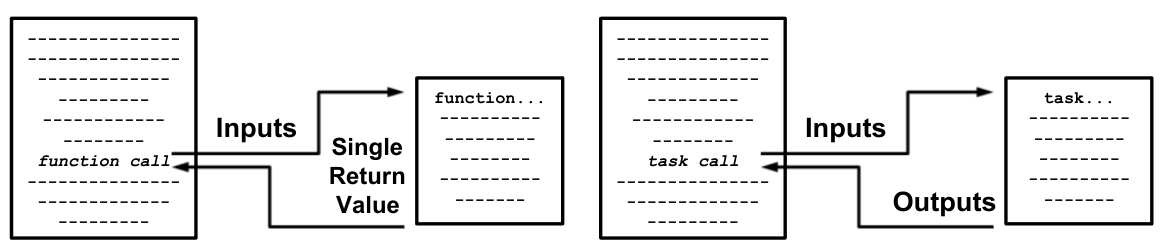
\includegraphics[width=0.95\textwidth]{img/10_subroutines.png}
\end{figure}
\end{frame}
\note{
\scriptsize{
Let's first examine the purpose of subroutines:
\begin{itemize}
\item We can think of a subroutine as a level of hierarchy, or structure, in sequential code. We can use subroutines to encapsulate some frequently used code in one place where we can more easily manage it. We can provide this ode with inputs, wo which we assign values as we invoke the subroutines. These input values can flexibly direct the subroutine to perform slightly for each invocation.

Encapsulating sequential code in subroutines is similar to encapsulating design units in modules.
\end{itemize}

}
}

%%%%%%%%%%%%%%%%%%%%%%%%%%%%%%%%%%%%%%%%%%%%%%%%%%%%%%%%%%%%
\begin{frame}[fragile]
\frametitle{Declaring Functions}
\scriptsize{
Function are declared only within a module. They start with \textcolor{purple}{function} keyword and ends with \textcolor{purple}{endfunction} keyword.
\newline

\textbf{Syntax:}
}
\tiny{
\begin{Verbatim}[commandchars=\\\{\}, tabsize=2]
\textcolor{purple}{function} [automatic] [signed] [range_or_type] function_identifier;
	tf_input_declaration;
	\{tf_input_declaration;\}
	\{block_item_declaration\}
	function_statement
\textcolor{purple}{endfunction}
\end{Verbatim}
}
\scriptsize{
\textbf{Alternative Syntax:}
}
\tiny{
\begin{Verbatim}[commandchars=\\\{\}, tabsize=2]
\textcolor{purple}{function} [automatic] [signed] [range_or_type] function_identifier;
	(function_port_list);
	\{block_item_declaration\}
	function_statement
\textcolor{purple}{endfunction}
\end{Verbatim}
}
\scriptsize{

\vfill
Function syntax without and with the function port list:
}
\begin{figure}
    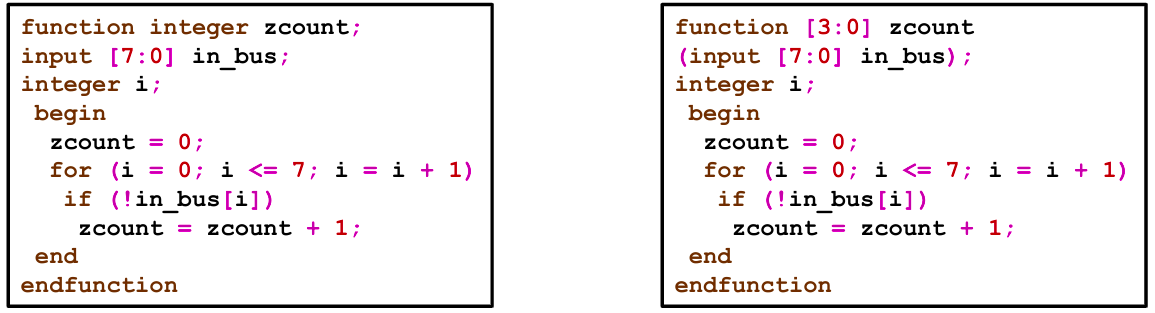
\includegraphics[width=0.95\textwidth]{img/10_function.png}
\end{figure}

\end{frame}
\note{
\tiny{
We declare a function only within a module. The declaration starts with the \textit{function} keyword.
\newline

Functions are by default \textbf{static}. That means that exactly one copy of the function variables exists. All calls to the function utilize that one set of function variables, thus calls to static functions are generally not recursive. External code can access static function variables using hierarchical references. Verilog 2001 added the \textit{automatic} declaration. Automatic functions create a new temporary set of their variables for each call. Automatic functions can be recursive. External code cannot access automatic function variables. The \textit{return} type defaults to a single bit. We can alternatively specify \textit{integer, real, realtime, time} or a vector range. A vector is by default not signed. We can declare the vector \textit{signed}. The signed declaration is a Verilog 2001 feature.
\newline

A function must have at least one input port and most have no output and no inout ports. We can declare input ports using either syntax. With the \textit{function port list} syntax, we can prefix port attributes. The input port defaults to the single bit. We can alternatively specify \textit{integer, real, realtime, time} or vector range. A venctor is by default not signed. We can declare the vector \textit{signed}. The signed declaration is a Verilog 2001 feature.
\newline

We can declare additional block items. We cannot declare module items. For example, we can declare variables but not nets!
\newline

A function declaration contains a statement. The statement may be a statement block, for example grouped between \textbf{begin} and \textbf{end} keywords. Functions cannot invoke the scheduler. That means that function assignments are always blocking and functions always execute completely and instantly.
\newline

Function can have side-effects, for example, a function can assign to a module variable but not to a module net. For a function to have side-effect is undesirable programming practice. Instead, declare the function return vector sufficiently wide to hold all data we need to return , then deconstruct the vector value as needed upon return.
\newline

A function declaration ends with the \textit{endfunction} keyword.

}
}

%%%%%%%%%%%%%%%%%%%%%%%%%%%%%%%%%%%%%%%%%%%%%%%%%%%%%%%%%%%%
\begin{frame}[fragile]
\frametitle{Calling Functions}
We call a function as an expression term:
\begin{Verbatim}[commandchars=\\\{\}, tabsize=2]
\textcolor{purple}{		function_identifier (expression \{, expression\})}
\end{Verbatim}
\begin{figure}
    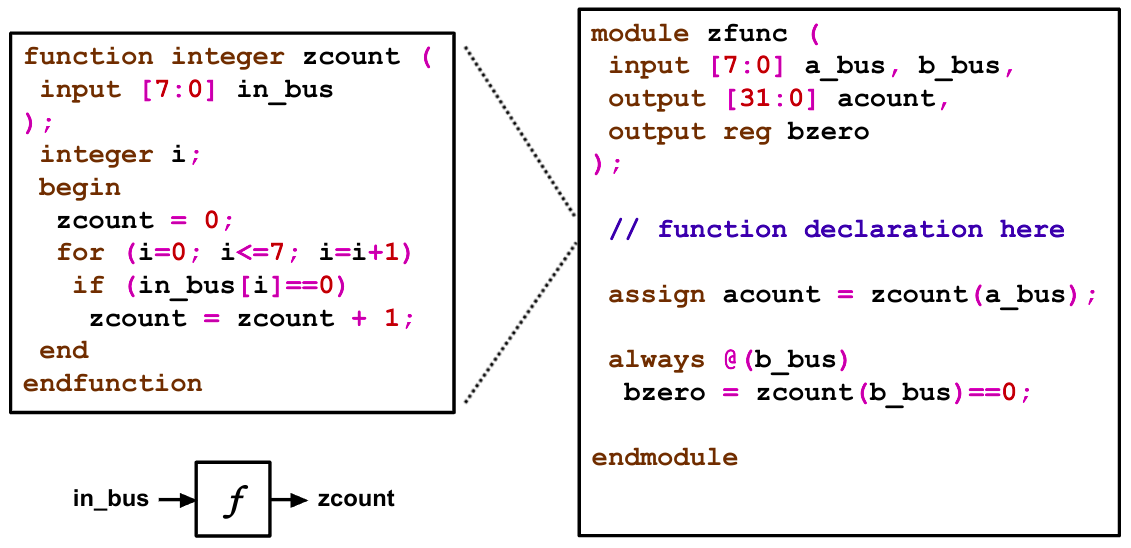
\includegraphics[width=0.95\textwidth]{img/10_function_call.png}
\end{figure}
\end{frame}
\note{
\scriptsize{
We call a function as an expression term. The simulator assigns the values of the argument expressions to the input ports in the order in which they appear in the call.
\newline

When the function completes, the simulator uses the value of the function name variable where the function call appears in the calling expression. Functions return a single value that we use as an operand in an \textit{rvalue} expression. An rvalue expression is one that may appear only on the right side of an assignment - we cannot assign a value to an rvalue expression. If the function never completes, for example, it executes a loop that loops forever, it never returns and simulator "hangs".
\newline

In this example, the \textit{zcount} function returns an integer value representing the number of bits of the \textit{in\_bus} port that are zero. It returns a value between 0 and 8. The continuous assignment call assigns the returned value to the \textit{acount} module output port. The procedural assignment call uses the function return value as an operand in a comparison expression.

}
}

%%%%%%%%%%%%%%%%%%%%%%%%%%%%%%%%%%%%%%%%%%%%%%%%%%%%%%%%%%%%
\begin{frame}
\frametitle{Constant Functions}
\scriptsize{
\begin{multicols}{2}
Verilog-1995 allows simple constant expressions for defining limits for vectors, replicates, etc.

\begin{itemize}

\item Verilog-2001 allows limits to be defined by constant functions.
\item Function value must be calculable at elaboration. Usually inputs are constants.
\item Greater flexibility for scalable reusable models.
\item Multiple limits can be derived from a single constant.
\end{itemize}
\vfill
\columnbreak
\begin{figure}
    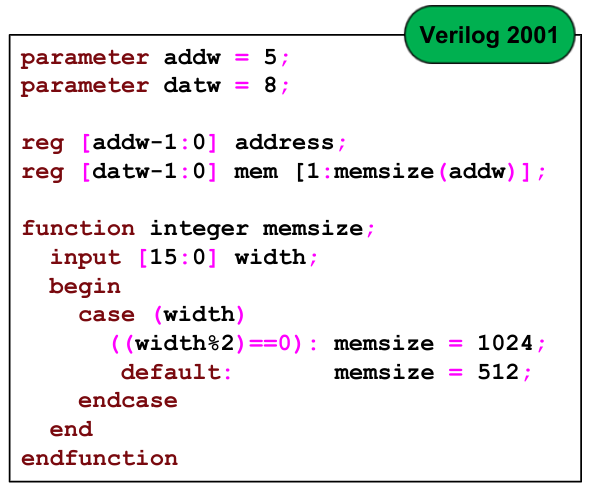
\includegraphics[width=0.45\textwidth]{img/10_function_const.png}
\end{figure}
\end{multicols}
}
\end{frame}
\note{
\tiny{
Verilog 1995 module parameter values must be constant expressions, which are limited to operations on literals and previously declared module parameters.
\newline

Verilog 2001 permits us to use a constant function call anywhere we are required to use a constant expression.
\newline

The standard lists restrictions upon a constant function calls:
\begin{itemize}
\item Cannot be placed within any generate scope
\item Cannot contain hierarchical references
\item Cannot contain system function calls 
\item Ignores system task calls (but will execute \$display in sumulator but not in elaborator)
\item Cannot themselves make constant function calls in any context requiring constant expressions. Can otherwise make constant function calls to functions local to containing module.
\item Can access only functions and module parameters and nothing else declared outside the function definition
\item Module parameters must be previously assigned. Use of \textit{defparam} can produce undefined results.
\end{itemize}

}
}

%%%%%%%%%%%%%%%%%%%%%%%%%%%%%%%%%%%%%%%%%%%%%%%%%%%%%%%%%%%%
\begin{frame}
\frametitle{Declaring Tasks}

\end{frame}

%%%%%%%%%%%%%%%%%%%%%%%%%%%%%%%%%%%%%%%%%%%%%%%%%%%%%%%%%%%%
\begin{frame}
\frametitle{Module}

\end{frame}

%%%%%%%%%%%%%%%%%%%%%%%%%%%%%%%%%%%%%%%%%%%%%%%%%%%%%%%%%%%%
\begin{frame}
\frametitle{Module}

\end{frame}

%%%%%%%%%%%%%%%%%%%%%%%%%%%%%%%%%%%%%%%%%%%%%%%%%%%%%%%%%%%%
\begin{frame}
\frametitle{Module}

\end{frame}

%%%%%%%%%%%%%%%%%%%%%%%%%%%%%%%%%%%%%%%%%%%%%%%%%%%%%%%%%%%%
\begin{frame}
\frametitle{Module}

\end{frame}

%%%%%%%%%%%%%%%%%%%%%%%%%%%%%%%%%%%%%%%%%%%%%%%%%%%%%%%%%%%%
\begin{frame}
\frametitle{Module}

\end{frame}

%%%%%%%%%%%%%%%%%%%%%%%%%%%%%%%%%%%%%%%%%%%%%%%%%%%%%%%%%%%%
\begin{frame}
\frametitle{Module}

\end{frame}

%%%%%%%%%%%%%%%%%%%%%%%%%%%%%%%%%%%%%%%%%%%%%%%%%%%%%%%%%%%%
\begin{frame}
\frametitle{Module}

\end{frame}

%%%%%%%%%%%%%%%%%%%%%%%%%%%%%%%%%%%%%%%%%%%%%%%%%%%%%%%%%%%%
\begin{frame}
\frametitle{Module}

\end{frame}

%%%%%%%%%%%%%%%%%%%%%%%%%%%%%%%%%%%%%%%%%%%%%%%%%%%%%%%%%%%%
\begin{frame}
\frametitle{Module}

\end{frame}

%%%%%%%%%%%%%%%%%%%%%%%%%%%%%%%%%%%%%%%%%%%%%%%%%%%%%%%%%%%%
\begin{frame}
\frametitle{Module}

\end{frame}

%%%%%%%%%%%%%%%%%%%%%%%%%%%%%%%%%%%%%%%%%%%%%%%%%%%%%%%%%%%%
\begin{frame}
\frametitle{Module}

\end{frame}

%%%%%%%%%%%%%%%%%%%%%%%%%%%%%%%%%%%%%%%%%%%%%%%%%%%%%%%%%%%%
\begin{frame}
\frametitle{Module}

\end{frame}




\end{document}
